It is a natural idea to check if the Goddard-Henning conjecture holds for small graphs with
computational help. The main challenge in doing so is generating all planar triangulations
on $n$ vertices.

Avis \cite{algorithm} gave an algorithm for generating all $3$-connected triangulated disks without
too many repetitions. For phrasing this more precisely, we call $(G, v_1, \dots v_r)$
an \emph{$r$-rooted triangulation} if $v_1, \dots, v_r$ are vertices of a face in $G$, and $G$
can be embedded in the plane with the following properties.

\begin{enumerate}
  \item The outer face of $G$ is formed by $v_1, \dots, v_r$, and they appear in
  this clockwise order.
  \item All the interior faces are triangles.
\end{enumerate}

The algorithm generates all $3$-connected $r$-rooted simple triangulations of order $n$ exactly once.
In this chapter, we will describe how this algorithm works.

To avoid a trivial case, suppose that $r < n$.

\begin{remark}
  Every $r$-rooted triangulation has a unique embedding to the plane in the sense that
  for every vertex $v$, the order of its neighbors is the same in all embeddings.
\end{remark}

\begin{claim} \label{c:3conn}
  An $r$-rooted triangulation is $3$-connected if and only if there exist no edges
  between two non-consecutive vertices of the outer face.
\end{claim}
\begin{proof}
  If there is an edge between two non-consecutive vertices of the outer face, then
  the endpoints of this edge clearly define a cut of the graph, so it is not $3$-connected.

  On the other hand, if $G = (V, E)$ is not $3$-connected, then there exist $u, v \in V$ such that
  removing $\{u, v\}$ from $G$, cuts the graph into $2$ parts. As $r$-rooted triangulations
  do not have cutting vertices, $u$ and $v$ must be on the outer face of $t$ and they
  are not consecutive to each other.
\end{proof}

The idea of the algorithm is as follows. First we construct an auxiliary graph $H = (T, F)$, where
$T$ is the set of $3$-connected $r$-rooted planar triangulations of order $n$. Then we
show that $H$ is connected. Finally, we perform a depth-first-search on $H$. For doing so,
we need to introduce a few notions first.

\begin{definition}
  We call an edge of a planar graph \emph{internal}, if it is not on the outer face of the graph.

  Let $t$ be an $r$-rooted triangulation and let $uv$ be an internal edge of $t$. There exist two
  faces containing $uv$: $uvx$ and $uvy$. We say that $uv$ is a \emph{transformable edge}
  if and only if $xy$ is not an edge in $t$.

  If $uv$ is transformable, we refer to the following operation as \emph{flipping} $uv$:
  delete the edge $uv$ and add the edge $xy$ to the graph. We denote the resulting
  graph with $flip(t, uv)$.

  We define the edge set of $H$ as follows. For $t_1, t_2 \in T$, $t_1t_2 \in F$ if and only
  there exists a transformable edge $e$ in $t_1$ such that $t_2 = flip(t_1, e)$.
\end{definition}

\begin{remark}
  $H$ is a well-defined undirected graph.
\end{remark}
\begin{proof}
  Suppose that $t_2$ can be obtained from $t_1$ by flipping
  $uv$ by adding the edge $xy$. Note, that $xy$ cannot be on the outer face of $t_2$.
  $uv$ is not an edge in $t_2$, so $xy$ is transformable, and flipping $xy$ results
  in the graph $t_1$.
\end{proof}

To prove the connectivity of $H$, we need the following lemma.

\begin{lemma} \label{l:trans}
  Let $v$ be a vertex in a $3$-connected $r$-rooted triangulation $G$. Suppose that $v$ is of degree
  at least $4$ and has at least one neighbor on the outer face of $G$. If $u_1, u_2, u_3, u_4$
  are consecutive neighbors of $v$ such that $u_1$ is on the outer face an $u_2$
  is not, then at least one of $vu_3$ and $u_2u_3$ is a transformable edge. Furthermore,
  the graph obtained by the transformation is also a $3$-connected $r$-rooted triangulation.
\end{lemma}
\begin{proof}
  $v_u3$ in an internal edge bounding faces $vu_2u_3$ and $vu_3u_4$. If $vu_3$
  is not transformable, then $u_2u_4$ is an edge. It is an internal edge, since $u_2$
  does not lie on the outer face. Let $xu_2u_4$ and $yu_2u_4$
  be the two faces bounded by $u_2u_4$. One of them must lie inside the triangle $vu_2u_4$,
  the other one must lie outside of it. ($v$ might be $x$ or $y$.) Thus, $u_2u_4$
  is transformable. (See Figure \ref{fig:trans}.)

  By Claim \ref{c:3conn}, to prove that the resulting graph is $3$-connected, it
  is enough to show that the new edge has an internal vertex.
  If $u_2u_4$ is the new edge, then $u_2$ is an internal
  vertex. Otherwise, the new edge is $xy$. One of them lies inside the $vu_2u_4$,
  and hence it is internal.
\end{proof}

\begin{figure}[ht]
  \centering
  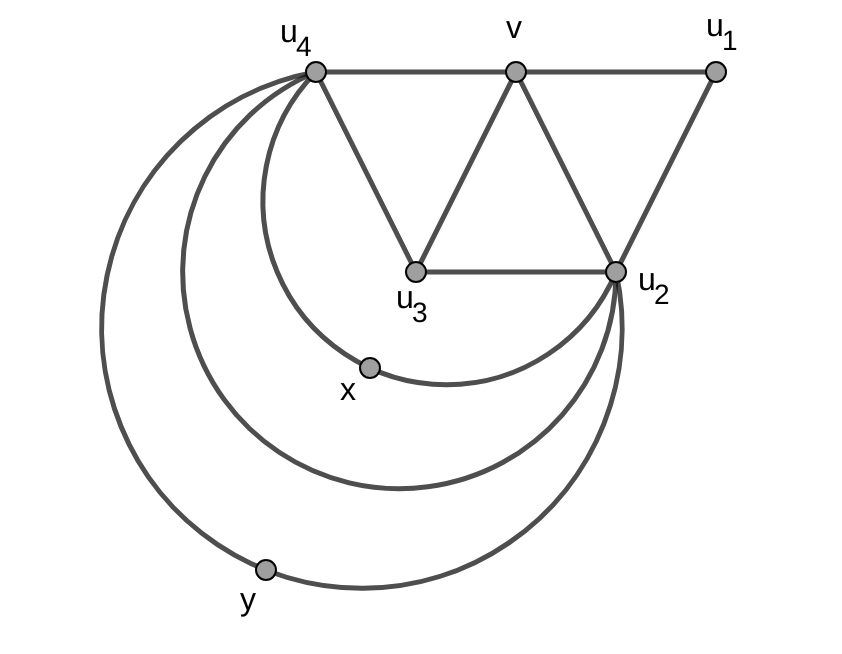
\includegraphics[width=70mm]{trans}
  \caption{Lemma \ref{l:trans}}
  \label{fig:trans}
\end{figure}

\begin{thm}
  $H$ is connected.
\end{thm}
\begin{proof}
  The proof goes as follows. First, we fix an $r$-rooted triangulation $t^*$. Then
  for every $t \in T$, we construct a path starting from $t$. Finally,
  we show that each of these paths ends in $t^*$.

  Define $t^*$ as follows. Let $v_1, v_2 \dots, v_r$ form the outer face of $t^*$.
  Connect $v_{r+1}$ to all the vertices of the outer face. For $i \ge r + 2$,
  put $v_i$ on the $v_{r-1}v_rv_{i-1}$ face and connect it with all of these three vertices.
  (See figure \ref{fig:root}.)

  \begin{figure}[ht]
    \centering
    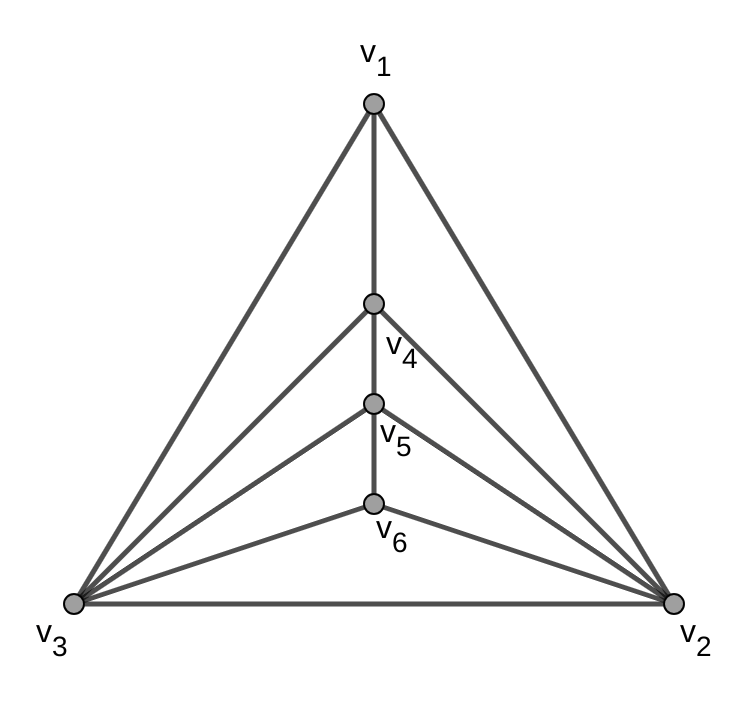
\includegraphics[width=70mm]{root}
    \caption{$t^*$ for $r=3$, $n = 6$}
    \label{fig:root}
  \end{figure}

  Let $t = (G, v_1, \dots v_r)$ be an $r$-rooted triangulation. We show now that
  Algorithm \ref{alg:path} stops in finitely many steps and constructs a path
  starting in $t$ and ending in $t^*$. Note, that when the algorithm flips an
  edge, then it is really transformable.
  \begin{algorithm}
    \caption{Construct path} \label{alg:path}
    \begin{algorithmic}
      \linespread{1.0}
      \small{
      \STATE let $p$ be an array of length $n$ /* $p[i]$ will be the $i^{th}$ vertex of the path.
      \STATE $p[0] := t$
      \WHILE{\TRUE}
        \STATE $j := j + 1$
        \STATE $i := 1$
        \WHILE{$deg(v_i) = 3$ and $i \le r - 2$}
          \STATE $i := i + 1$
        \ENDWHILE
        \IF{$i \le r - 2$}
          \STATE /* The outer face of $t$ differs from the outer face of $t^*$.
          \STATE let $v_{i - 1}, u_2, u_3, u_4$ be consecutive neighbors of $v_i$ in
          counterclockwise order
          \IF{$u_2u_4 \not\in E$}
            \STATE $p[j] := flip(t, v_iu_3)$
          \ELSE
            \STATE $p[j] := flip(t, u_2u_4)$
          \ENDIF
        \ELSE
          \STATE /* The outer face looks good, identify the possible $v_{r+1}$.
          \STATE let $w$ be the vertex connected to $v_1, \dots v_{r - 2}$.
          \STATE $a = v_1$
          \WHILE{$w$ has exactly one neighbor $b \neq a$ not on the outer face of  $t$}
            \STATE /* If $w$ was the possible $v_k$, then $b$ is the possible $v_{k + 1}$.
            \STATE $a = w$
            \STATE $w = b$
          \ENDWHILE
          \IF{$deg(w) = 3$}
            \STATE return $p$
          \ELSE
            \STATE let $v_r, u_2, u_3, u_4$ be consecutive neighbors of $w$ in
            counterclockwise order
            \IF{$u_2u_4 \not\in E$}
              \STATE $p[j] := flip(t, wu_3)$
            \ELSE
              \STATE $p[j] := flip(t, u_2u_4)$
            \ENDIF
          \ENDIF
        \ENDIF
        \STATE $t := p[j]$
      \ENDWHILE}
    \end{algorithmic}
  \end{algorithm}
  \linespread{1.3}


  We claim that after enough steps, $deg(v_1) = \dots = deg(v_{r - 2}) = 3$.
  Otherwise, $deg(v_i) \neq 3$ for some $i \le r - 2$. Let $i$ be the smallest such index.
  Then the algorithm takes $v_{i - 1}, u_2, u_3, u_4$ such that they are consecutive neighbors of $v_i$
  in counterclockwise order. If $v_iu_3$ is transformable, then the degree of $v_i$
  decreases and for every $j < i,$ $deg(v_j)$ does not change. Suppose that $v_iu_3$
  is not transformable. Then let $xu_2u_4$ and $yu_2u_4$ be the two faces bounding $u_2u_4$.
  Suppose $y = v_j$ for some $j < i$. From $deg(v_j) = 3$ it follows, that $u_4$ must be $v_{j - 1}$.
  On the other hand, by $3$-connectivity, if $u_4$ is an external vertex, then it
  is $v_{i + 1}$ and hence $i = r - 1$, which is a contradiction. So adding $xy$ to the graph
  does not change the degree of $v_j$ for any $j < i$. In the next step of the algorithm,
  $v_iu_3$ is transformable. Thus, we showed, that after enough steps, $deg(v_i) = 3$ for every $i \le r - 2$.

  If $v_1, \dots v_{r - 2}$ are all degree $3$ vertices, then there exists a vertex $w$
  such that $w$ is connected to $v_1, \dots v_r$. If $w$ has
  more than one internal neighbor, than the algorithm chooses $v_r, u_2, u_3, u_4$ to
  be consecutive neighbors of $w$ in counterclockwise order. If $wu_3$ is transformable,
  then the algorithm deletes $wu_3$ from the graph and adds $u_2u_4$ to it. By executing this step,
  the degree of $w$ decreases, and for $j \le r - 2$, $deg(v_j)$ does not change.
  The other case is when $wu_3$ is not transformable. Let $x$ and $y$ be the
  vertices of the two faces bounded by $u_2u_4$, In this case the algorithm
  deletes $u_2u_4$ from the graph and adds $xy$ to it. This does not change the
  degree of $v_j$ for $j \le r - 2$. In the next step of the algorithm $wu_3$ is
  transformable. Thus, after some steps, $w$ will have only one internal neighbor $b$.
  It follows, that $bv_r$ and $bv_{r - 1}$ are edges. With the same process, we
  achieve that $b$ has at most $1$ internal neighbor apart from $v$. It is easy to see, that
  the changes do not affect vertices outside of $bv_rv_{r - 1}$. Therefore, by iterating these
  steps we can achieve $t^*$.
\end{proof}

The proof shows that by performing a depth-first-search on $H$, one
can generate all $r$-rooted $3$-connected triangulations. To determine the neighbors
of a triangulation $t \in H$, we check for each edge $e$ in $t$ if $e$ is transformable in $t$.
For each pair $(t, e)$, this can be done in $O(n)$ time. Hence, if
$K$ denotes the number of all $r$-rooted $3$-connected triangulations on $n$ vertices, then
the algorithm finishes in $O(n^2K)$ time.
